% Chapter 1

\chapter{Theory} % Main chapter title

\label{Chapter2} % For referencing the chapter elsewhere, use \ref{Chapter1} 

This chapter outlines the theoretical aspects of this study, covering both the linear wave theory used in the wave model and the theory behind data assimilation methods. The aim is to give the reader an overview of all the theory needed to understand the methods and results of the study.

\section{Ocean Waves}

Ocean waves are a distinctive visual feature of the ocean surface, and very important to offshore operations such as wind farms. This section will describe some of the physical processes influencing ocean waves, as well as the theory of linear waves and wave energy spectra as as modelled by the WAVEWATCH III (WW3) model used in this project \citep{WW3DG2019}.

\subsection{Physical Processes}

Ocean waves are an instance of surface gravity waves, meaning they propagate on the interface between two fluids of different densities. Their restoring force is gravity. The focus of this project is on waves with periods from ~10s - ~0.25s, which are generated by wind, although ocean waves can exist on a wide range of scales and be influenced by other factors such as surface tension and local air pressure variations
\citep[pp. 3-7]{Holthuijsen2007}. 

There are multiple hypothesised physical mechanisms for the generation of waves by wind. \citet{Phillips1957} shows that small-scale turbulent eddies induce small surface waves at frequencies matching the frequency of the turbulence. \citet{Miles1957} describes how the surface height variations from these small waves lead to energy transfer from the wind to the waves, thus increasing wave height. A more detailed overall description of the various processes is given in \citet{Janssen2004}, chapter 3.

The wind almost always acts as a source of wave energy, so there has to be a process present to dissipate waves and act as an energy sink. These processes are poorly understood but \citet{Janssen2004}, section 4.9 describes multiple physical mechanisms which may contribute to wave dissipation. One important process affecting dissipation is wave breaking, which occurs in near shorelines when the wave height gets too large compared to the water depth. It can also occur when wave height gets too large compared to wavelength. This steepness induced breaking is also known as white capping. Water's molecular viscosity can lead to the damping of shorter waves and larger waves can be damped by the surface eddies induced by wave breaking.

Ocean waves in deep water are dispersive, and waves with longer wavelengths travel faster than waves with shorter wavelengths (discussed quantitatively in section \ref{sec:linwaves}). This leads to a phenomenon known as swell, which is the name given to long waves that have travelled far from their source. Due to dispersion these waves have no short-wavelength component, so swell waves have longer wavelengths and periods than waves near the site of generation which are affected by local winds (known as wind sea). The other feature of swell waves is their regular appearance. While a wind sea has wave components in many different directions, by the time the waves have travelled away from the source these different components will spread out so that they do not overlap, and the resulting swell will be almost unidirectional. See figure \ref{fig:windandswell} for a schematic.

\begin{figure}
\centering
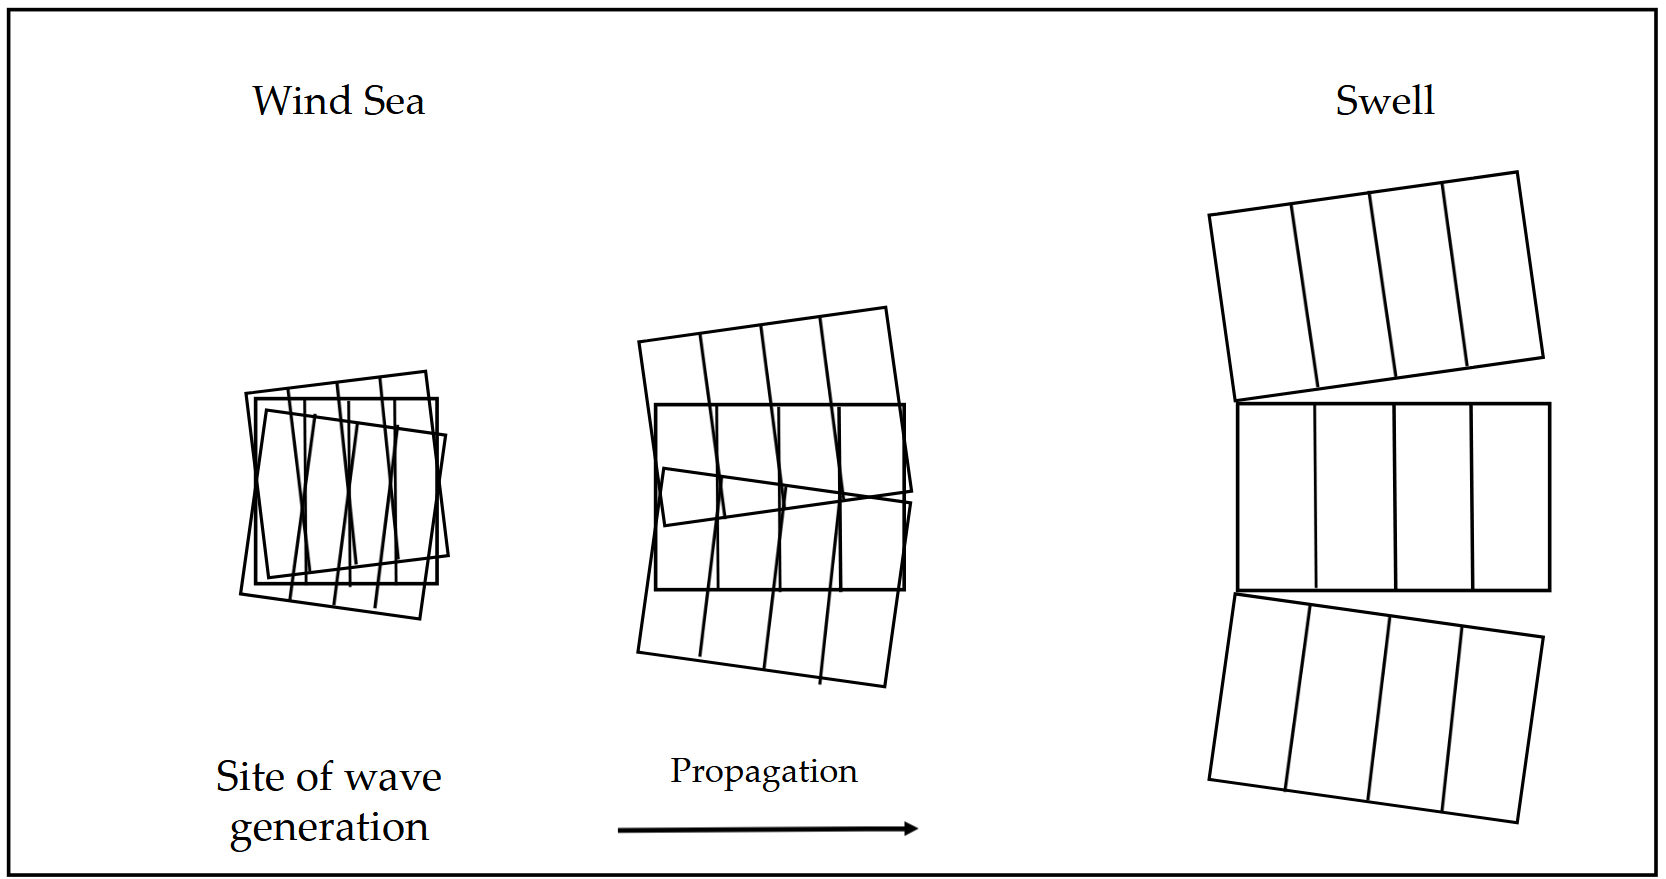
\includegraphics[width = 0.8\textwidth]{Figures/windandswell}
\caption{Schematic of the generation of wind and swell waves.}
\label{fig:windandswell}
\end{figure}

\subsection{Linear Wave Theory}
\label{sec:linwaves}

This section will outline the linear wave theory relevant to this project, as derived in \citet{Vallis2017}, page 253. Linear wave theory is an approximation, and other higher-order theories of surface gravity waves exist, such as Stokes waves and cnoidal waves \citep{Osborne2010}. These higher-order theories will not be considered here since the WAVEWATCH III (WW3) model used in this project models the ocean surface as a linear superposition of simple linear waves.

Parameters describing linear waves include the wavenumber $k$, direction $\theta$ and frequency $\omega$. The first two describe the wave vector $\vect{k}$, which has magnitude $k$ and direction $\theta$,

\begin{equation}
\vect{k} = - k \sin \theta \uvec{\imath} - k \cos \theta \uvec{\jmath},
\end{equation}

where  $\uvec{\imath},\uvec{\jmath}$ are unit vectors pointing East and North respectively. \comment{}{Make bold if you can}. Note that $\theta$ measures the wave direction in the meteorological convention i.e. the direction the wave is coming from. This means that $\theta = 0 \degrees$ corresponds to a \replace{N}{n}ortherly wave, $\theta = 90\degrees$ corresponds to an \replace{E}{e}asterly wave and so on, and is the same convention used in WW3.

Here, $\omega$ denotes the absolute frequency measured in a fixed frame of reference. If the medium is subject to currents, this will differ from the relative frequency $\sigma$ measured in a frame of reference moving with the mean current, due to the Doppler effect. This difference is quantified by the equation

\begin{equation}
    \omega = \sigma + \vect{k} \cdot \vect{U},
    \label{eqn:doppler}
\end{equation}

where $\vect{U}$ is the mean current vector. $\sigma$ and $k$ are related by the dispersion relation

\begin{equation}
    \sigma^2 = gk\tanh{kD},
    \label{eqn:disprel}
\end{equation}

where $D$ is the water depth. The dispersion relation has two limiting forms:

\begin{itemize}
    \item Deep water waves, where $kD \gg 1$, so $\tanh{kD} \approx 1$ and $\sigma^2 \approx gk$.
    \item Shallow water waves, where $kD \ll 1$, so $\tanh{kD} \approx kD$ and $\sigma^2 \approx gk^2D$.
\end{itemize}

The phase speed is then given by

\begin{equation}
c = \frac{\sigma}{k} \approx \begin{cases}
            \sqrt{\frac{g}{k}} &\text{in deep water}, \\
            \sqrt{gD} &\text{in shallow water},
\end{cases}
\label{eqn:pspeed}
\end{equation}

and the group speed may be expressed as

\begin{equation}
c_g = \frac{\partial\sigma}{\partial k} = \frac{1}{2}c \left(1 + \frac{2kD}{\sinh{2kD}} \right) \approx \begin{cases}
    \frac{1}{2} c &\text{in deep water}, \\
    c &\text{in shallow water}.
\end{cases}
\label{eqn:gspeed}
\end{equation}

The phase speed is the speed at which the wave peaks and troughs move, whereas the group speed is the speed at which wave groups move. The group speed is then the speed at which energy is transported by the wave. The wave travels in the direction of the wave vector $\vect{k}$ so the group and phase velocities are given by

\begin{align*}
\vect{c}& = - c \sin\ \theta \uvec{\i} - c \cos \theta \uvec{\j}, \\
\vect{c}_g& = - c_g \sin \theta \uvec{\i} - c_g \cos \theta \uvec{\j}.
\end{align*}

We can now use scale analysis to see that $\omega$ and $\sigma$ generally have similar values. The ratio between $\vect{k}\cdot\vect{U}$ and $\sigma$ in equation \ref{eqn:doppler} is

\[
\frac{\vect{k}\cdot\vect{U}}{\sigma} \sim \frac{kU}{\sigma} = \frac U c,
\]

where $U = |\vect{U}|$ is the mean current speed. Since $c \gg U$ in general, this ratio is small and so $\omega \approx \sigma$.

\subsection{Wave Spectra}
\label{sec:wavespectra}

Note that equations \ref{eqn:doppler} - \ref{eqn:gspeed} are valid for linear waves of a single frequency and direction. Real ocean waves are more complicated than this, containing multiple frequencies propagating in multiple directions. The WAVEWATCH III (WW3) model used in this project models ocean waves as a superposition of these simple linear waves.

Surface waves with multiple frequencies and directions are represented using a wave spectrum $F = F(\sigma,\theta)$, which is also a function of position and time. $F$ represents the sea surface height variance associated with a particular frequency $\sigma$ and direction $\theta$, so the total height variance is 

\begin{equation}
\overline{\eta^2} = \iint F \intd\sigma \intd\theta.
\label{eqn:waveenergy}
\end{equation}

This is related to the wave energy per unit surface area $E$ via $E = \rho g \overline{\eta^2}$. A rigorous definition of $F$ is given in \citet{Holthuijsen2007}, section 3.5.6. One can also define the direction-integrated spectrum $S(\sigma) = \int F(\sigma,\theta) \intd\theta$, which quantifies the surface height variance as a function of frequency. This can be integrated to calculate the energy contained in a specific frequency band $\Delta \sigma$:

\begin{equation}
\Delta E = \rho g \int_{\Delta \sigma} S(\sigma) \intd\sigma.
\end{equation}

$S$ is a helpful diagnostic from which information about the appearance of the waves can be inferred. A widely spread spectrum implies irregular waves with many different frequency components whereas a tight spectrum implies regular waves with one dominant frequency. Low frequency waves correspond to swell, while high frequency waves correspond to a wind sea. An example of a direction-integrated spectrum is plotted in figure \ref{fig:examplespec}. This spectrum comes from a point in the GoM that is far from any shorelines. We can see two peaks on the spectrum, one at about 0.3 Hz which corresponds to wind waves and one at about 0.2 Hz, which corresponds to swell. The wide spread of this spectrum indicates that the waves probably have an irregular appearance.

\begin{figure}
\centering
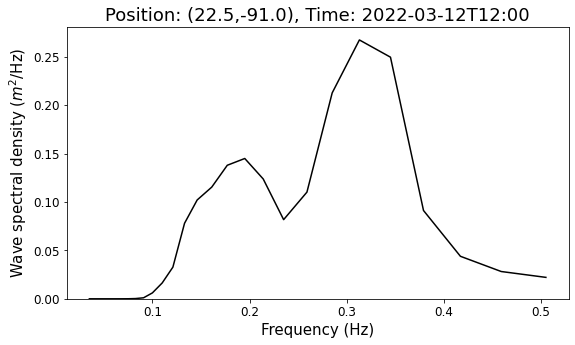
\includegraphics[width = 0.7\textwidth]{Figures/examplespec}
\caption{An example spectrum from a point in the gulf of Mexico. Calculated from WW3 spectral forecast data.}
\label{fig:examplespec}
\end{figure}

Here, we also define the wave spectral moments which are derived from the direction-integrated spectrum:

\begin{equation}
m_k = \int S(\sigma) \sigma^k \intd\sigma, \quad m = \dots,-1,0,1,\dots .
\label{eqn:moments}
\end{equation}

Note that $m_0 = \overline{\eta^2}$ is the overall surface height variance. These moments give information about the statistical properties of the ocean, and can be used to derive other important wave variables from the spectrum. In this project we focus on the significant wave height $H_s$ and two measures of period $T_{m01}$, $T_{m02}$. \citet{Holthuijsen2007}, section 4.2 (in which significant wave height is denoted $H_{m0}$) gives derivations of these variables from the spectral moments, reproduced below:

\begin{align}
H_s &= 4\sqrt{m_0}, \\
T_{m01} &= \frac{m_0}{m_1}, \\
T_{m02} &= \sqrt{\frac{m_0}{m_2}}.
\label{eqn:mainvars}
\end{align}

$T_{m01}$ is the mean wave period, that is the reciprocal of the mean frequency of the wave spectrum, and $T_{m02}$ is the mean zero-crossing period, that is the average period between times when the wave-induced surface height displacement crosses zero. Finally we define the wave action

\begin{equation}
N(\sigma,\theta) = \frac {F(\sigma,\theta)} {\sigma}.
\label{eqn:waveaction}
\end{equation}

$N$ is conserved in the absence of sources and sinks \parencite{Bretherton1968}, so it very useful for wave modelling. WW3 works by evolving the wave action according to the effects of sources and sinks (see section \ref{sec:model}).

\section{Data Assimilation}

Data assimilation (DA) refers to a group of statistical methods for incorporating observations into forecasts. It requires a model state and some observations, and the assumption that the observations are a function of some underlying true state of the system. The goal is to find the state that is most likely given the forecast and observation data, assuming some distributions for the errors in each.

\subsection{Vector Representations and Cost Function}
\label{sec:DAintro}

In DA, the state of a system must be represented with a vector so that methods of linear algebra can be applied to it. This section covers some of the details of this, as well as the treatment of observations and basic method by which the most likely state is found.

We take a vector $\x \in \mathbb{R}^n$ to represent the state of the system. This state is represented computationally in a model, and the form of $\x$ depends on the DA application. In some cases, $\x$ simply has one component for each variable of the system at each model gridpoint. Other applications use what is known as an augmented or 4D state vector, where $\x$ is expanded to contain components from times $t = 0,1,\dots,T$ i.e.

\[
\x = \begin{pmatrix} \x (t = 0) \\ \x (t = 1) \\ \vdots \\ \x (t = T) \end{pmatrix}.
\]

An augmented state vector is used in this study. Given a first guess $\x_b$, we assume that the state of the system has a normal distribution $\prob(\x) = N(\x_b,\mat{B})$. $\x_b$ here is called the background state, and is usually taken to be the state of the model before DA is applied. $\mat{B}$ is called the background error covariance matrix. Since the true background error covariance matrix is generally unknown, it must be estimated, and methods of achieving this are discussed later.

We take a vector $\y \in \mathbb{R}^p$ to represent a set of observations, and assume $\y$ is related to $\x$ via an observation operator $\mathcal{H}: \mathbb{R}^n \rightarrow \mathbb{R}^p$ and an error term $\varepsilon$,

\[
\y = \mathcal{H}(\x_\text{true}) + \varepsilon,
\]

where $\x_\text{true}$ is the unknown true state of the atmosphere. The error term $\varepsilon$ is assumed to be normally distributed with mean zero and covariance $\mat{R}$: $\varepsilon \sim N(0,\mat{R})$. The matrix $\mat{R}$ is referred to as the observation error covariance matrix.

We call the vector spaces containing $\x$ and $\y$ the state space and observation space respectively. In most operational contexts, the dimensions of these spaces are very large: $\x$ has at least one component for each variable involved in the assimilation at each model gridpoint, so typically $n \sim 10^8$. $\y$ has at least one component for each observed variable at each observation location, so $p \sim 10^6$. This means that considerable computational resources are required in most cases and computational efficiency is a key consideration in any operational DA implementation.

In our case, we have three variables on a $181 \times 210$ grid and each forecast window contains 169 timesteps, so the dimension of our state space is approximately $2 \times 10^7$. We have only one observation location measuring the same three variables and we assimilate observations from 73 different timesteps, so the dimension of the observation space here is only 219. Note that these dimsensions are smaller than those seen in operational contexts, so the DA problem is smaller with fewer degrees of freedom. This means that solving it computationally is practical on the hardware accessible in this study. Further details and motivation for these numbers are given in section \ref{sec:DAsetup}.

In our case $\mathcal{H}$ is linear, that is, there is a matrix $\mat{H} \in \mathbb{R}^{n \times p}$ such that $\mathcal{H}(\x) = \mat{H}\x$, and so the probability distribution of $\y$ given that the system is in state $\x$ is $\prob(\y|\x) = N(\mat{H}\x,\mat{R})$. We can then express the distribution of $\x$ given some set of observations $\y$ using Bayes' theorem:

\begin{equation}
    \prob(\x|\y) = \prob(\y|\x) \frac{\prob(\x)}{\prob(\y)}.
\end{equation}

This allows $\prob(\x|\y)$ to be determined since $\prob(\y|\x)$ and $\prob(\x)$ are known, and $\prob(\y)$ is independent of $\x$ so it acts as a normalisation constant. Since all the distributions involved are normal, $\prob(\x|\y)$ will be normally distributed also,

\begin{equation}
    \prob(\x|\y) = A(\y) e^{-\frac 1 2 \left( \norm[\mat{B}^{-1}]{\x - \x_b}^2 + \norm[\mat{R}^{-1}]{\y - \mat{H}\x}^2\right)},
\label{eqn:xgiveny}
\end{equation}

adopting the notation $\norm[\mat{M}]{\vect{a}}^2 = \vect{a}^\top \mat{M} \vect{a}$. $A(\y)$ in this equation is a normalising constant whose value is chosen so that the integral of $\prob(\x|\y)$ over all values of $\x$ is equal to 1 for each $\y$.

We then seek the most likely value i.e. the mode of this distribution, since this will be a good estimate for the true state of the system given background state $\x_b$ and observations $\y$. Finding the mode of equation \ref{eqn:xgiveny} is equivalent to minimising a cost function

\begin{equation}
    J(\x) = \frac 1 2 \norm[\mat{B}^{-1}]{\x - \x_b}^2 + \frac 1 2 \norm[\mat{R}^{-1}]{\y - \mat{H}\x}^2.
    \label{eqn:cost3d}
\end{equation}

The first term of \ref{eqn:cost3d} represents the deviation of $\x$ from the background state and the second term represents the deviation from the observations, with the overall cost function being a sum of these two weighted by the background and observation error matrices. This means that when the background error is large compared to the observational error, the observations will be given more weight and vice versa.

\subsection{Kalman Filters}
\label{sec:kalmanfilters}

The specific DA method used in this study is based on the ensemble transform Kalman filter, which is part of a broad class of methods called Kalman filters. This section begins with a discussion of the overall properties of Kalman filters, followed by a more specific description of ETKF and the method used in this study.

The state that minimises the cost function in equation \ref{eqn:cost3d} is called the analysis $\x^a$ and may be expressed as

\begin{equation}
    \x^a = \x_b + \mat{K}\vect{d}^o_b
\label{eqn:analysisupdate}
\end{equation}

where $\vect{d}^o_b = \y - \mat{H}\x_b$ is the innovation and $\mat{K} = \mat{B}\mat{H}^\top\left(\mat{H}\mat{B}\mat{H}^\top + \mat{R}\right)^{-1}$ is the Kalman gain (derived in \citet{Asch2016}, pp. 92-96).

Note that the increment $\vect{d}^a_b = \x^a - \x_b$ is given by $ \mat{B}\left(\mat{H}^\top\left(\mat{H}\mat{B}\mat{H}^\top + \mat{R}\right)^{-1} \vect{d}^o_b \right)$, so it always lies in the column space of $\mat{B}$. This means that $\mat{B}$ is crucial to determining how information from the observations is spread around the domain by the DA system. In particular, if $\mat{B}$ is rank deficient, then all possible increments lie within a strict subspace of the state space. This reduces the degrees of freedom in the corrections the DA system can make, which can limit the performance of the system.

One class of DA methods which use equation \ref{eqn:analysisupdate} are called Kalman filters, in which context it is called the analysis step. Kalman filters alternate this analysis step with a forecast step in which a forecast model is used to evolve the state forward to the next observation time. Kalman filters approximate $\mat{B}$ with a flow-dependent error covariance matrix $\mat{P}$ (equations \ref{eqn:ferrorcov} and \ref{eqn:aerrorcov}) which is explicitly part of the DA output and which is evolved forward in time by the model along with the state. Kalman filters are a broad class of methods, with many variants existing \citep{Evensen1992,Bishop2000,Hunt2007,Houtekamer2016}.

In this project we borrow the Kalman filter analysis step, also known as the update step, to update the model state. Our method is not strictly speaking a Kalman filter since we do not have access to the forecast model, which means we are unable to perform the forecast step required in a Kalman filter method. This process of using the forecast model to evolve the DA corrections forward to the next assimilation time is called cycling, and is a central part of most DA systems. We view the fact that we are unable to do this as an important limitation of this study.

To get around the lack of cycling, we instead make use of a single analysis step to update an entire 7-day forecast window at once. This requires augmenting the state vector to include components from each leadtime within the window, which brings the dimension of the state space up to $\sim 2 \times 10^7$. We also augment the observation vector to include observations from each observation time. Since we are assimilating observations from the first three days of each window, the dimension of the observation space becomes 219.

It is important to note that this process of simultaneously assimilating observations from different times means that the method used in this study is not a filter method, since filter methods by definition assimilate observations sequentially according to the time the observations were taken. Methods in which observations from different times are assimilated simultaneously are called smoothers. The method used here, in which a Kalman filter analysis step is used to assimilate observations from a whole window of times, is quite an unconventional smoother implementation, and more conventional methods such as 4DVar and 4DEnVar are described in \citet{Bannister2017}.

The specific method whose analysis step we borrow is called the ensemble transform Kalman filter (ETKF). The implementation we use is from the parallel data assimilation framework (PDAF), described in section \ref{sec:DAsetup}. The choice of method was motivated partially by the fact that the availability of the PDAF routine makes implementation easier, and partially by the fact that the ETKF is computationally efficient compared to many other DA methods \citep{Hunt2007}. The ETKF implementation provided by PDAF is based on the LETKF method described in \citet{Hunt2007}, without applying localisation. \citet{Asch2016} gives a thorough description of the method, which is outlined here.

In the ETKF method, the analysis is performed in ensemble subspace rather than in the state space. Algebraically this means expressing the increment as a linear combination of ensemble perturbations

\begin{align}
\mat{X}_f &= \frac{1}{\sqrt{N- 1}} \left( \x^f_1 - \overline{\x}^f, \x^f_2 - \overline{\x}^f, \dots, \x^f_N - \overline{\x}^f \right),  \label{eqn:ensperturbations}\\
\x^a &= \overline{\x}^f + \mat{X}_f \vect{w}^a, \label{eqn:ensspaceupdate}
\end{align}

where $\x^f_i$ is the state of ensemble member $i$ prior to assimilation and the ensemble mean $\overline{\x}^f$ is used as the background state. The columns of $\mat{X}^f$ are the perturbations of each ensemble member from the ensemble mean, and $\vect{w}^a$ is a coefficient vector which determines the weighting of each ensemble perturbation in equation \ref{eqn:ensspaceupdate}. From \citet{Asch2016} pp.163-164, the optimal coefficient vector $\vect{w}^a$ is given by

\begin{equation}
\vect{w}^a = \left( \mat{I}_N + \mat{X}_f^\top \mat{H}^\top \mat{R}^{-1} \mat{H} \mat{X}_f \right) ^{-1} \mat{X}_f^\top \mat{H}^\top \mat{R}^{-1} \vect{d}^o_b,
\label{eqn:ETKFinc}
\end{equation}

where $\vect{d}^o_b = \y - \mat{H} \overline{\x}^f$. This method is algebraically equivalent to performing the analysis step in state space (equation \ref{eqn:analysisupdate}) with background state $\overline{\x}^f$ and background error covariance matrix given by the forecast error covariance matrix

\begin{equation}
\mat{P}_f = \mat{X}_f \mat{X}_f^\top .
\label{eqn:ferrorcov}
\end{equation}

This matrix is rank deficient since its column space has dimension equal to the ensemble size, which limits the degrees of freedom of the increments as discussed earlier. Indeed, this limitation can also be seen directly from equation \ref{eqn:ensspaceupdate}, since the vector $\vect{w}^a$ is in the ensemble space which has dimension equal to the number of ensemble members and much less than the dimension fo the state space. This method was chosen nonetheless since according to \citet{Hunt2007}, working in ensemble space has considerable advantages over working in state space in terms of computational cost.

Note that this method only gives a single analysis state, where we started with an ensemble. To get a full analysis ensemble, we first define the analysis error covariance matrix, which is prescribed by Kalman theory \citep[section 3.4.3]{Asch2016} to be 

\begin{equation}
\mat{P}^a = \left( \mat{I}_n - \mat{KH} \right) \mat{P}^f .
\label{eqn:aerrorcov}
\end{equation}

Here $n$ is the dimension of state space as before. In this case the Kalman gain matrix takes the form $\mat{K} = \mat{P}^f\mat{H}^\top \left(\mat{HP}^f\mat{H}^\top + \mat{R} \right)^{-1}$. To generate the analysis ensemble, we need to factorise $\mat{P}^a$ to get the analysis ensemble perturbations $\mat{P}^a = \mat{X}_a\mat{X}_a^\top$. We can rewrite equation \ref{eqn:aerrorcov} as

\begin{align*}
\mat{P}^a &= \left( \mat{I}_n - \mat{X}_f \mat{X}_f^\top \mat{H}^\top \left(\mat{HP}^f\mat{H}^\top + \mat{R} \right)^{-1} \mat{H} \right) \mat{X}_f \mat{X}_f^\top \\
&= \mat{X}_f \left( \mat{I}_N - \mat{X}_f^\top \mat{H}^\top \left(\mat{HP}^f\mat{H}^\top + \mat{R} \right)^{-1} \mat{H} \mat{X}_f \right) \mat{X}_f^\top,
\end{align*}

so we define $\mat{X}_a$ as

\begin{equation}
\mat{X}_a = \mat{X}_f \left( \mat{I}_N - \mat{X}_f^\top \mat{H}^\top \left(\mat{HP}^f\mat{H}^\top + \mat{R} \right)^{-1} \mat{H} \mat{X}_f \right) ^{\frac 1 2}.
\end{equation}

The notation $\mat{A}^{\frac 1 2}$ here refers to the matrix square root, which is defined to be a matrix $\mat{B}$ such that $\mat{B}^\top\mat{B} = \mat{A}$. This definition is ambiguous since for any orthogonal matrix $\mat{U}$, $\mat{UB}$ is also a square root of $\mat{A}$. The method described in \citet{Hunt2007} takes the symmetric square root, which is uniquely defined by \citet{Horn2013}, theorem 7.2.6. A desirable property of this choice is that it leads to an unbiased filter, that is, the mean of the analysis ensemble is equal to the mean of the forecast ensemble \citep{Livings2008}.

\[
\mat{X}_a = \mat{X}_f \left( \mat{I}_N + \mat{X}_f^\top \mat{H}^\top \mat{R}^{-1} \mat{H} \mat{X}_f \right)^{-\frac 1 2}
\]

using the Sherman-Morrison-Woodbury identity \citep[p. 50]{Golub1996}. The full analysis ensemble can then be generated from the analysis state derived in equation \ref{eqn:ETKFinc} via

\begin{equation}
\x^a_i = \x^a + \sqrt{N-1} \mat{X}_f \left[ \left( \mat{I}_N + \mat{X}_f^\top \mat{H}^\top \mat{R}^{-1} \mat{H} \mat{X}_f \right)^{-\frac 1 2} \right]_i,
\label{eqn:ETKFens}
\end{equation}

where the notation $[\_]_i$ refers to the $i^\text{th}$ column of the matrix being taken. Now the analysis ensemble perturbations match exactly the form of the forecast ensemble perturbations,

\begin{equation}
\mat{X}_a = \frac{1}{\sqrt{N- 1}} \left( \x^a_1 - \x^a, \x^a_2 - \x^a, \dots, \x^a_N - \x^a \right),
\end{equation}

since the $i^\text{th}$ column of $\mat{X}_a$ is

\begin{align*}
\left[ \mat{X}_a \right]_i &= \mat{X}_f \left[ \left( \mat{I}_N + \mat{X}_f^\top \mat{H}^\top \mat{R}^{-1} \mat{H} \mat{X}_f \right)^{-\frac 1 2} \mat{U} \right]_i \\
&= \frac{1}{\sqrt{N-1}} \x^a - \x^a_i.
\end{align*}\

\subsection{Practical Aspects}
\label{sec:DApractice}

In this section, we discuss some of the pitfalls that can arise when implementing the ETKF, along with potential solutions. It is important to note that none of the solutions discussed here are implemented in this study, for the sake of computational simplicity and for other reasons discussed later in the section. Description of them is included nonetheless as knowledge of the potential problems helps to explain the results of this study, and the solutions are useful to inform future work.

When calculating $\mat{P}^f$ from the ensemble, spurious covariances may arise at long distances \citep{Hunt2007}, especially when the ensemble size is small. This is problematic as it can lead to large increments far from observation locations, which is physically unrealistic. One way to fix this is called localisation, and involves multiplying each element of the forecast error covariance matrix $\mat{P}^f_{ij}$ by a factor which depends on the distance between gridpoints $i$ and $j$. Representing this distance with $d(i,j)$, we define the matrix $\mat{D}$ by $\mat{D}_{ij} = f(d(i,j))$ for some function $f: \mathbb{R}^+ \rightarrow [0,1]$ of our choosing. We then define the new error covariance matrix $\mat{P}^{f\prime}$ via the following equation:

\begin{equation}
\mat{P}^{f\prime} = \mat{P}^f \circ \mat{D}.
\end{equation}

So the localisation effectively scales the covariance values by a factor between 0 and 1 determined by the function $f$, the aim being to suppress the spurious long-distance covariances. Here $\circ$ denotes the Schur product of the two matrices, that is $\mat{P}^{f\prime}_{ij} = \mat{P}^f_{ij} \mat{D}_{ij}$.

The choice of $f$ is important as it determines the nature of the localisation. In particular, $f$ should be close to 1 when $d(i,j)$ is small and close to 0 when $d(i,j)$ is large, to suppress covariances at long distances while allowing them to exist at short distances. \citet{Hunt2007} gives a detailed description of the local ensemble transform Kalman filter (LETKF) obtained by applying localisation to the ETKF. In that study, $f$ is chosen by setting a cutoff radius $r$ and defining $f$ by

\[
f(d) = \begin{cases}
	1, \quad &d < r, \\
	0, &r \leq d.
\end{cases}
\]

It also possible to make $f$ a continuous function such that given in \citet{Gaspari1999}:

\[
f(d) = \begin{cases}
	- \frac 1 4 \left(\frac d r \right)^5 + \frac 1 2 \left(\frac d r \right)^4 + \frac 5 8 \left(\frac d r \right)^3 - \frac 5 3 \left(\frac d r \right)^2 + 1, &0 \leq d \leq r, \\
	 \frac{1}{12} \left(\frac d r \right)^5 - \frac 1 2 \left(\frac d r \right)^4 + \frac 5 8 \left(\frac d r \right)^3 + \frac 5 3 \left(\frac d r \right)^2 - 5 \left(\frac d r \right) + 4 - \frac 2 3 \left(\frac d r \right)^{-1}, \quad &r \leq d \leq 2d, \\
	0, &2d \leq r,
\end{cases}
\]

where $r$ is a cutoff radius as before. This form of $f$ has been successfully applied to EnKF and other methods in multiple studies, such as \citet{Hamill2001,Houtekamer2001,Whitaker2002}.

Another advantage of localisation in the context of the ETKF is that is goes some way to solve the problem of rank deficiency. The matrix $\mat{D}$ is full rank so the forecast error covariance matrix after localisation $\mat{P}^{f\prime} = \mat{P}^f \circ \mat{D}$ is full rank also, as opposed to $\mat{P}^f$ which is rank deficient. Thus localisation increases the degrees of freedom in the DA increments, which has the potential to improve DA performance at the cost of increased computational expenditure.

No localisation is implemented in this study. This a partly to maintain computational simplicity as much as possible, and partly because in the examination of the forecast error covariances in section \ref{sec:bgerrors} we find some long-distance covariances that do not appear to be spurious. Excluding these potentially physically realistic long-distance covariances may have a detrimental impact on DA performance, so we go with the simpler option and do not include any localisation.

Another problem that may be encountered is $\mat{P}^f$ being an underestimate of the true background error covariance. This is a result of sampling error that affects the estimation of $\mat{P}^f$ from the ensemble \citep{Sacher2008}. This alone is not necessarily undesirable, since it will lead to the analysis covariance $\mat{P}^a$ being smaller which reduces spread in the analysis ensemble. Ensemble spread is a commonly used metric of forecast uncertainty, so some reduction in spread is desirable. 

It is possible for $\mat{P}^f$ to be too small, however, as by equation \ref{eqn:cost3d} a small $\mat{P}^f$ leads to increments which are erroneously small, and tends to compound over multiple analysis steps since a tighter analysis ensemble leads to a smaller forecast error covariance matrix at the next analysis step, which leads to a problem called filter divergence (\citet{Jazwinski1970}, pp.301-305). Note that in our case it will not compound since we are only doing one analysis step per model run, but it should be checked that the increments are realistic and the analysis ensemble spread is not too small even after one analysis step.

This can be tested by comparing the analysis ensemble to the true value. If the truth lies outside the range given by the ensemble spread, then the ensemble spread is too small and we say the ensemble is `overconfident'. A schematic is shown in figure \ref{fig:ensconfidence}. The ensemble on the left has appropriate spread, as the ensemble mean lies within the range given by the ensemble. The ensemble on the right is overconfident, as the range of the ensemble is too small to capture the truth.

Note that we do expect the truth to lie outside this range sometimes, as we expect the ensemble values to be randomly distributed around the true value. However, a high prevalence of overconfident ensembles is undesirable, since as mentioned before, ensemble spread is commonly used to estimate uncertainty in a forecast. Overconfident ensembles may lead to too much confidence being placed in an incorrect forecast, which is detrimental to any decision making that is informed by the forecast.

Various methods are available to counteract this problem, but one of the simplest is called inflation \citep{Anderson1999}. This involves multiplying the forecast error covariance matrix $\mat{P}^f$ by a predefined factor $\alpha > 1$ prior to the analysis step. This increases the size of the increments that may be applied by the system, and also increases the spread of the analysis ensemble, which reduces overconfidence.

As with localisation, we do not apply any inflation in this study. This choice was informed by preliminary DA experiments with no inflation in which the relation between forecast error and ensemble spread seemed appropriate.

\begin{figure}[h]
\centering

\includegraphics[width = .6\textwidth]{figures/ensconfidence}
\caption{Left: an ensemble with appropriate spread. Right: an overconfident ensemble. Truth is shown in black, ensemble mean and spread is shown in blue and ensemble members are shown in green.}
\label{fig:ensconfidence}
\end{figure}

\section{Chapter Summary}

This chapter was intended to give an overview of the theoretical aspects of this study. We have seen details of ocean wave theory, including qualitative descriptions of physical mechanisms affecting waves and quantitative treatments of the linear theory and wave spectra used in WAVEWATCH III. A description of DA theory has been given, from the basic aspects of state vectors and cost functions to a more specific description of Kalman filters and some potential problems that can arise when using these methods.

Particular attention has been given throughout to the topics most relevant to this study, such as the ETKF method which is borrowed heavily from. It is hoped that the theory presented in this chapter provides a basis for understanding the methods and results presented in the subsequent chapters of this study.
